\marginpar{§\ref{ch:creativity}}

\nameref{ch:creativity}

\hyperlink{refname}{something}
\hypertarget{refname}{something else}

It's also possible to link directly any word or
\hyperlink{thesentence}{any sentence} in you document.

For instance \hypertarget{thesentence}{this sentence}.



\begin{fcom}
  noise\\
  basins of attraction\\
  break symmetry\\
  creativity is not linear\\
  phase shift\\
  \autocite{Everitt2011}
\end{fcom}

\todo{golden compass, paulman?}

``Traversing the representations of this ambiguity using algorithms inspired by the syzygy, clinamen and anomaly of pataphysics, using a panalogical mechanism applied to metadata, should be able to humanize and even poeticize the experience of searching the Web.'' \autocite{Hendler2013}

% marvosym
\Forward
\MoveDown
\RewindToIndex
\ToTop
\ForwardToEnd
\MoveUp
\RewindToStart
\ForwardToIndex
\Rewind
\ToBottom

% bclogo
\bcloupe

% fontawesome
\faicon{search}
\faicon{info}
\faicon{comment-o}
\faicon{eye}
\faicon{table}
\faicon{code}
\faicon{object-group}
\faicon{bookmark-o}
\faicon{picture-o}




% \begin{quotation}
%   ``Observation as a method for data collection raises issues as to its reliability in creativity evaluation. Data from observing creativity depends upon the interpretation of what the individual observer sees.'' \sourceatright{\autocite[p.22]{Candy2012}}
% \end{quotation}



\begin{quote}
  ``The participant responses demonstrate active engagement in three ways: Immediate, Sustained or Creative.'' \autocite{Candy2012}
\end{quote}

\begin{quote}
  ``Whether an action is successful or unsuccessful depends on whether the intended result is achieved.'' \autocite[p.23]{Candy2012}
\end{quote}

\begin{quote}
  ``Also, evaluation of novelty (or originality, newness) is often examined in the papers cited above according to how dissimilar the system’s artefacts are to previous output or other existing examples of creative output in that domain. On the other hand, appropriateness is often evaluated according to how similar the system’s output artefacts are to known examples. Hence across the field as a whole, there is a stark inconsistency as to whether to prioritise the generation of artefacts which are dissimilar from existing artefacts, or whether to pursue the generation of artefacts which are similar to existing artefacts, arising directly from the adoption of ‘novelty + value’ as the underlying model of creativity. Such a contradiction is clearly not helping the identification of coherent and consistent strategies to adopt across the field.'' \autocite{Jordanous2012}
\end{quote}

\begin{quote}
  ``In some cases, evaluative tests are conducted on the system which purportedly evaluate the system’s creativity but which actually only measure the system’s quality.'' \autocite{Jordanous2012}
\end{quote}

\begin{draft}
  But if quality is the ``conformance to specifications'' and the specification suggested creativity, then a good quality rating of a system would automatically mean it's creative, right?
\end{draft}



\begin{landscape}
\begin{table}[htb]
  \begin{tabu}{XXXXXX}
  \toprule
  \textbf{Novelty}
  &
  \textbf{Value}
  &
  \textbf{Quality}
  &
  \textbf{Ephemeral \newline Uncontrolled}
  &
  \textbf{Temporal \newline Controlled}
  &
  \textbf{Purpose}
  \\ \midrule
  Originailty
  &
  Usefulness
  &
  Skill
  &
  Serendipity
  &
  Persistence
  &
  Intention
  \\ \midrule
  Newness
  &
  Appropriateness
  &
  Efficiency
  &
  Randomness
  &
  Results
  &
  Communication
  \\ \midrule
  Variety
  &
  Appreciation
  &
  Competence
  &
  Uncertainty
  &
  Development
  &
  Evaluation
  \\ \midrule
  Typicality
  &
  Relevance
  &
  Intellect
  &
  &
  Progression
  &
  Aim
  \\ \midrule
  Imagination
  &
  Impact
  &
  Acceptability
  &
  &
  Spontaneity
  &
  \\ \midrule
  &
  Influence
  &
  &
  Experimentation
  &
  &
  Independence
  \\
  \bottomrule
  \end{tabu}
\caption[Creativity attributes]{Summary of all creativity attributes}
\label{creatt}
\end{table}
\end{landscape}









@book{Hugill2012,
  author = {Hugill, Andrew},
  booktitle = {Philosophy},
  publisher = {Self},
  title = {{Lineaments of 'Pataphysics}},
  year = {2012}
}

% Introduction
\begin{tikzpicture}[
    decoration={
    reverse path,
    text along path,
    text path start scale=1.5,
    % text path start scale=3,
    text path end scale=0,
    text={Feeling a movement of pity, discovered the induction coil, cette irraisonnee induction, and entered the opening in the wall. Only by some recherche movement, apres coup et sous forme d'introduction, opening his seized manuscript, the enemy made within the enclosure of the vineyard. Which he had thrown off at the beginning of his labor, in opening so exactly at the, than the thirst of my paternity. We can then start at once, and whose informing voice had consigned me to the hangman, as any person at all conversant with authorship may satisfy himself at.}}
]
\draw [decorate]
    (0.8\textwidth, 0) % horizontal. circle then line to side
    % (0, 0.5\textwidth) % vertical. line from top down to circle
    % \foreach \i [evaluate={\r=(\i/2000)^2}] in {0,5,...,2880}{ -- (\i:\r)};
    \foreach \i [evaluate={\r=(\i/2500)^2}] in {0,10,...,3500}{ -- (\i:\r)};
\useasboundingbox (-2.75,-2.75) rectangle (2.75,2.75);
% \useasboundingbox (-5,-5) rectangle (5,5);
\end{tikzpicture}

% \begin{tikzpicture}
% \draw [domain=0:25.1327,variable=\t,smooth,samples=55]
%     plot[mark=*,mark options={fill=white}] ({\t r}: {0.002*\t*\t});
% \end{tikzpicture}

``These types of results are incredably useful for any one who derives value from new ideas.''\autocite{Yossarian2015}

In regards to my project:
\begin{itemize}
  \item A concept implementation method is used with a descriptive-other approach
  \item A qualitative investigation into if and why the proposed search results are useful will be done
  \item Following experimental methodologies, to evaluate the proposed new solution to the problem of creative search
\end{itemize}


bridge: how do current search engines work? they prioritise revelvance using pagerank algorithms etc. happens at crawling time. pataphysics isnt about relevance. (index is ranked)

pataphysics cant be ranked. need for neutrality in index but creative ways to retrieve matches for query.
but then changed to focus on the concept of searching/browsing (in itself, rather than part of a system architecture) and ranking as a creative process.
pataphysicalisation happens at query time between query and index. (index is neutral)

project was to build a prototype that proves these ideas.
my eventual approach was to take elemnts from both the ontology idea and the relevance ranking IR way and combine/redeploy them in a new way using pataphysics that would yield results designed to foster/inspire creativity.

% \begin{quote}
%   ``One way of characterizing these processes is to use an alliteration that allows us to keep track of some of the core features of RRI in ICT, namely the four `p's, which are: product, process, purpose and people. The purpose of using the four `p's is to draw attention to the fact that, in addition to the widely recognized importance of both product and process of technical development, the purpose of the development needs to be considered and people involved in the innovation need to be incorporated in RRI [Responsible Research and Innovation].'' \autocite{Stahl2013}
% \end{quote}

\begin{fcom}
  poems = combinatorial creativity visualised.
  From calculated relevance to creative detour.
\end{fcom}



\grule

% NOTES

\begin{quote}
  ``Whatever the context, evaluation is always tailored to the approach, needs, purpose and methodology of that context.'' \autocite[p.7]{Candy2012}
\end{quote}

\begin{quote}
  ``The matrix for evaluating creativity represents three standpoints: the capabilities of the creator, the audience, or more accurately, participant, experiences, and the features of the interactive systems as artworks. This initial matrix has been extended to include creative processes for both creator and audience participant (i.e.\ working practices and interaction experiences) and contextual factors in the form of the physical and technical environment in which the creative acts and events take place, including the influence of physical and technical resources and real world constraints.'' \autocite[p.7-8]{Candy2012}
\end{quote}

\begin{quote}
  ``The evaluation of user, or rather, participant, experience of interactive artworks often involves measurement of aesthetic appreciation and the various engagement qualities which are dependent on personal traits, motivations, expectations, emotions and cognitive states of the audience. Those experiences that involve open-ended activity tend towards the creative end of human activity and, as such, are hardly ever measurable in quantitative ways.''  \autocite[p.8]{Candy2012}
\end{quote}

\begin{quote}
  ``Evaluation is a key activity in creative design that can be revealed through documentation from design rationale. The introduction of rationale has been an important contribution to the quest for clarity and traceability in design decision-making. Design rationale may be thought of as structured records of design that support the understanding of decisions taken and allow designers to give better informed reconsideration to them at a later stage.'' \autocite[p.9]{Candy2012}
\end{quote}

\begin{quote}
  ``A software system can be viewed as an artifact that embodies implicit theoretical constructs that are realized as functional and operational requirements (Carroll and Campbell 1989). Structures are chosen because of their ability to achieve the intended functionality, and such choices may be evaluated against various criteria. During the design process, the ideas are modified and there is a clarification and refinement of intended functions and features. There may be additional factors arising from the context of the project that affect the way the design is carried out: for example the need to keep sight of general applicability whilst meeting the domain specific requirements, or the influence of the given hardware platform and software tools. Whatever the situation, the relationship between designers' decision making and the design outcome is not necessarily transparent and this is can be a problem when it comes to system maintenance. The explicit listing of decisions made during a design process, and the reasons why those decisions were made provides a means to record and communicate the reasoning and justification behind a design decision, including alternatives considered and constraints that affected the decision-making including why alternatives were rejected. The successful application of design rationale to software system design can provide a form of communication of intent from the designer to those who are to maintain the system.'' \autocite[p.9]{Candy2012}
\end{quote}

\begin{quote}
  ``A promising approach to the externalization of decision-making during the design process is being explored within practice-based research in the creative arts in the form of documented reflective practice. The approach builds upon a normal part of creative practice whereby practitioners draw and note ideas, designs and options in their sketch and notebooks. In this way, the documentation of tentative ideas and how they are worked into firmer proposals through testing and evaluation is a familiar and integral part of creativity. In practice-based research, documented reflective practice and empirical studies are frequently brought together.'' \autocite[p.10]{Candy2012}
\end{quote}

\begin{quote}
  The Multi-dimensional Model of Creativity and Evaluation (MMCE) shown in Figure 1 has four elements: people, process, product and context. \autocite[p.11]{Candy2012}
\end{quote}

\begin{figure}[htb] % (here, top, bottom, page)
  \centering
  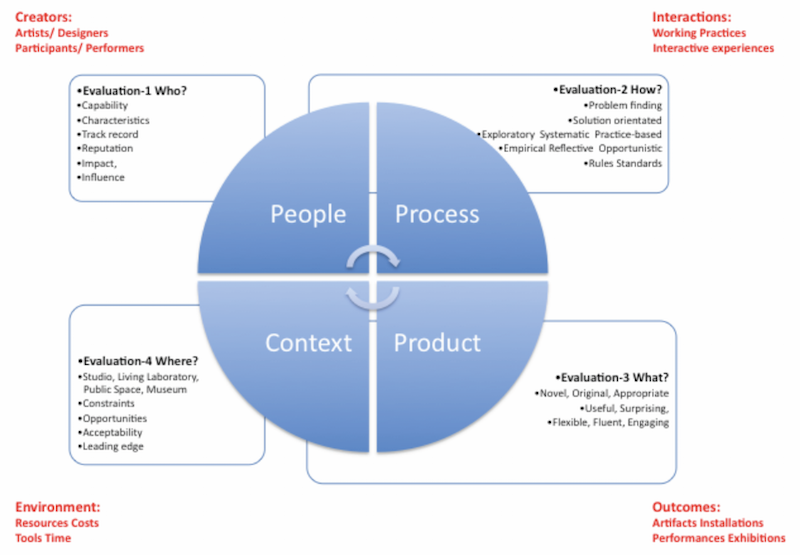
\includegraphics[width=\linewidth]{images/candy02.png}
\caption[Multi-dimensional Model of Creativity and Evaluation]{Candy's Multi-dimensional Model of Creativity and Evaluation}
\label{fig:candy02}
\end{figure}

\begin{figure}[htb] % (here, top, bottom, page)
  \centering
  \includegraphics[width=\linewidth]{images/candy01.png}
\caption[Text for Table of Contents]{Caption text under figure}
\label{fig:candy01}
\end{figure}

\textbf{PEOPLE AS CREATORS}: \autocite[p.14-15]{Candy2012}

Criteria for evaluating creator capability:
\begin{enumerate}
  \item The creator must be able to demonstrate an ability to create an artistic outcome where subject matter, ideas and technique are combined well to produce a coherent outcome.
  \item The creator must be able to demonstrate an ability to make work that is exploratory, creative and imaginative. Interesting ideas are presented in intelligent and surprising ways.
  \item In respect of Composition and Interpretation, the creator must be able to demonstrate the ability to:\\
  •	Select subject matter that is appropriate to a given theme\\
  •	Manipulate ideas and techniques in a coherent manner\\
  •	Express ideas visually (visual communication)\\
  •	Respond in an individual and personal way
\end{enumerate}

\textbf{PROCESS AS INTERACTION}: \autocite[p.17]{Candy2012}

Criteria for evaluation can be expressed as follows
1. For a work to be deemed engaging, the participant should exhibit observable responses. There are likely to be different levels of engagement depending on whether or not the audience has had prior experience of this kind of artwork or installation or similar.\\
2. The participant responses demonstrate active engagement in three ways: Immediate, Sustained or Creative. The categories are defined as follows:\\
•	Immediate engagement: the work grabs immediate attention and yet is not so mundane as to create boredom.\\
•	Sustained engagement: the work must excite curiosity in the and also be accessible to a general audience.\\
•	Creative engagement: the work must excite immediate attention and encourage an audience to interact with it in a playful/purposeful way. As attention declines with familiarity and time, changes take place in the work that renew audience engagement.

\textbf{PRODUCT AS OUTCOME}: \autocite[p.18]{Candy2012}

Typical features for judging artworks include composition, aesthetic, affect, content, and technique. Criteria for evaluation can be expressed as follows:

•	the composition of work should be coherent, exhibit shape and balance between order and complexity.\\
•	the work should exhibit outstanding visual and sound qualities in color, line and form.\\
•	the work should be pleasing, challenging, exciting, original etc.\\
•	the content should be appropriate and effective for the chosen subject matter\\
•	the execution should demonstrate high quality technique that fits the form.

It is interesting, therefore, to consider how criteria for judging the digital arts are specified by the Prix Ars Electronica, an international competition for Cyber Arts and the foremost event of its kind today.

Entries are judged by a Jury of experts in the order of their arrival and according to the following categories:

•	Aesthetics • Originality\\
•	Excellence of execution\\
•	Compelling conception\\
•	Innovation in technique of the presentation

\textbf{CONTEXT AS ENVIRONMENT}: \autocite[p.21]{Candy2012}

Establishing a workable living laboratory for interactive art and evaluation involved setting down acceptance criteria for assessing whether or not a new interactive art system was ready to be deployed.

These included:
•	degree of robu\\stness of the art system in expectation of heavy public use
•	appropriate accessibility in respect of type of audience (e.g.\ children)\\
•	adherence to safety and house rules required by the museum\\
•	impact of other coinciding exhibits (sound, noise, light impacts)\\
•	attention to participant orientation and training\\
•	attention to art system maintenance by creator and technical support

\begin{quote}
  ``we need to apply strategies for generating clear and unambiguous data that can be turned into meaningful information. From meaningful information, we can then derive understandings related to the context of use, the outcome of which might take the form of a coherent model.'' \autocite[p.21]{Candy2012}
\end{quote}

\begin{quote}
  ``Observation as a method for data collection raises issues as to its reliability in creativity evaluation. Data from observing creativity depends upon the interpretation of what the individual observer sees.'' \autocite[p.22]{Candy2012}
\end{quote}

\begin{quote}
  ``However, in order to ‘measure’ creativity, we have to conduct research outside of controlled laboratory conditions, and cannot rely on fixed criteria that can be applied to all cases. The shifting ground and the ever-changing contexts often renders consistency out of reach.'' \autocite[p.22]{Candy2012}
\end{quote}

\begin{quote}
  ``If the term `measurement' does not match what we are doing within the creativity domain, then why do we still use this word?'' \autocite[p.22]{Candy2012}
\end{quote}

\begin{quote}
  ``Whether an action is successful or unsuccessful depends on whether the intended result is achieved.'' \autocite[p.23]{Candy2012}
\end{quote}

\begin{quote}
  ``Measuring success is more likely to be dependent on factors such as whether or not the system has engaged the audience in a playful or immersive way or whether it has elicited curiosity or excitement or concentrated attention and so on.'' \autocite[p.23]{Candy2012}
\end{quote}


% -----------------------------

% \begin{fcom}
% •	Brain operations per sec 1016 \autocite[p.194]{Kurzweil2013}\\
% •	Japan’s K-computer has 1016 calculations per sec (10 petaflops)\\
% •	Blue brain project: 2023: 1017 bytes memory + 1018 flops \autocite[p.125]{Kurzweil2013}
% \end{fcom}
%
% Human Brain Project: \autocite{Walker2012}
%
% Our brain consumes about 30W, the same as an electric light bulb, thousands of times less than a small supercomputer. \autocite[p.17]{Walker2012}
%
% For environmental and business reasons, vendors have set themselves the goal of containing energy consumption to a maximum of 20 megawatts  \autocite[p.41]{Walker2012}
%
% the 1 PFlop machine at the Jülich Supercomputing Centre could simulate up to 100 million neurons – roughly the number found in the mouse brain. \autocite[p.41]{Walker2012}
%
% Cellular-level simulation of the 100 billion neurons of the human brain will require compute power at the exascale (1018 flops). \autocite[p.41-42]{Walker2012}
%
% 2017 petascale 50petabytes memory + 50 petaflops + <=4MW power
%
% 2021 exascale 200petabyte memory + 1exaflop
%
% A second, equally important goal will be to prepare the procurement of the HBP Pre-exascale-supercomputer. By 2017/18, Jülich plans to procure a Big Data-centred system with at least 50 PBytes of hierarchical storage-class memory, a peak capability of at least 50 PFlop/s and a power consumption <= 4 MW. The memory and computational speed of the machine will be sufficient to simulate a realistic mouse brain and to develop first-draft models of the human brain. (The rest of the hardware roadmap targets an exascale machine in 2021/2022 with a capability of 1 EFlop/s and a hierarchical storage-class memory of 200 PB).\footnote{https://www.humanbrainproject.eu/high-performance-computing-platform}
%
% Chris Chatham: 10 Important Differences Between Brains and Computers \footnote{http://scienceblogs.com/developingintelligence/2007/03/27/why-the-brain-is-not-like-a-co/}
%
% \begin{enumerate}
% \item Brains are analogue; computers are digital
% \item The brain uses content-addressable memory
% \item The brain is a massively parallel machine computers are modular and serial
% \item Processing speed is not fixed in the brain; there is no system clock
% \item Short-term memory is not like RAM
% \item No hardware/software distinction can be made with respect to the brain or mind
% \item Synapses are far more complex than electrical logic gates
% \item Unlike computers, processing and memory are performed by the same components in the brain
% \item The brain is a self-organising system
% \item Brains have bodies
% \item	The brain is much, much bigger than any [current] computer
% \end{enumerate}
%
% Why Minds Are Not Like Computers \autocite{Schulman2009}
% Software – Hardware == Mind – Brain ??? analogy
%
% "The power of the computer derives not from its ability to perform complex operations, but from its ability to perform many simple operations very quickly."
%
% Layers of abstraction in computers:\\
% 1.	user interface\\
% 2.	high level programming language\\
% 3.	machine language\\
% 4.	proessor microarchitecture\\
% 5.	Boolean logic gates\\
% 6.	transistors\\
%
% layers of abstraction in brain:\\
% 1.	personality?\\
% 2.	Thinking?\\
% 3.	Chemical /electrical signals/activity?\\
% 4.	Divided Brain regions/structure\\
% 5.	Neurons\\
% 6.	Dendrites (input) and axons (output)?\\
%
%
% Computers are faster and better than humans in many tasks already.
%
% \begin{quote}
% "The weaknesses of the computational approach include its assumption that cognition can be reduced to mathematics and the difficulty of including noncognitive factors in creativity." \autocite[p.457]{Mayer1999}
% \end{quote}
%
% \subsection{Other}
%
% \begin{quote}
% "Currently many implementors of creative systems follow a creative-practitioner-type approach: produce a system then present it to others, whose critical reaction determines its worth as a creative entity. A creative practitioner’s primary aim, however, is to produce creative work, rather than to critically investigate creativity; in general this investigative aim is important in computational creativity research." \autocite{Jordanous2011}
% \end{quote}
%
% purpose or intention shifts into focus here over production of products.
%
% \begin{quote}
% "Also, evaluation of novelty (or originality, newness) is often examined in the papers cited above according to how dissimilar the system’s artefacts are to previous output or other existing examples of creative output in that domain. On the other hand, appropriateness is often evaluated according to how similar the system’s output artefacts are to known examples. Hence across the field as a whole, there is a stark inconsistency as to whether to prioritise the generation of artefacts which are dissimilar from existing artefacts, or whether to pursue the generation of artefacts which are similar to existing artefacts, arising directly from the adoption of ‘novelty + value’ as the underlying model of creativity. Such a contradiction is clearly not helping the identification of coherent and consistent strategies to adopt across the field." \autocite{Jordanous2012}
% \end{quote}
%
% \begin{quote}
% "In some cases, evaluative tests are conducted on the system which purportedly evaluate the system’s creativity but which actually only measure the system’s quality." \autocite{Jordanous2012}
% \end{quote}
%
% But if quality is the "conformance to specifications" and the specification suggested creativity, then a good quality rating of a system would automatically mean it's creative, right?
%
% \begin{quote}
% "The key conclusion of the survey was that evaluation of computational creativity is not being performed in a scientifically rigorous manner:
% \begin{itemize}
% \item The creativity of a third of the 75 ‘creative’ systems was not critically discussed.
% \item Half the papers surveyed did not contain a section on evaluation.
% \item Only a third of systems presented as creative were actually evaluated on how creative they are.
% \item A third of papers did not clearly state or define criteria that their system should be evaluated by.
% \item Less than a quarter of systems applied existing creativity evaluation methodologies.
% \item Occurrences of evaluation by people outside the system implementation team were rare.
% \item Few systems were comparatively evaluated, to see if the presented system outperforms existing systems (a useful measurement of research progress).
% \item General principles of scientific method are not being followed by the community as a whole." \autocite{Jordanous2012}
% \end{itemize}
% \end{quote}
%
% \begin{quote}
% "Reducing creativity to problem solving works when the creator is searching for an ideal solution which is not obvious, or if there is no single ideal solution but several candidates for a reasonable solution (Boden, 1994b)." \autocite{Jordanous2012}
% \end{quote}
%
% \begin{quote}
% "One potential problem with Boden’s three views of creativity is that they all assume the existence of a conceptual space, or constrained set of possibilities, that the creative individual consciously reasons with in order to be creative." \autocite{Jordanous2012}
% \end{quote}

\begin{figure}[htb] % (here, top, bottom, page)
  \centering
  \includegraphics[width=\linewidth]{candy01}
\caption[Text for Table of Contents]{Caption text under figure}
\label{fig:candy01}
\end{figure}







``TD research therefore starts with a problem that is `in the world and actual' as opposed to `in my head and conceptual'.'' ``This inherent feature of `creating change' highlights the relevance of using the term `consequential' to characterise TD research approaches and problems.'' \autocite{Wickson2006}


% \textbf{Information System}
% "An information system is not the information technology alone, but the system that emerges from the mutually transformational interactions between the information technology and the organization." \autocite{Mingers2004}
%
% \textbf{Inductive reasoning}
% "is a kind of reasoning that constructs or evaluates general propositions that are derived from specific examples. Inductive reasoning contrasts with deductive reasoning, in which specific examples are derived from general propositions." [wikipedia]
%
% \textbf{Specific to General}
% In an inductive approach you "collect data and develop theory as a result of your data analysis." \autocite{Knox2004}
%
% \textbf{Deductive reasoning}
% "is the process of reasoning from one or more general statements regarding what is known to reach a logically certain conclusion." [wikipedia]
%
% \textbf{General to Specific}
% In a deductive approach you "develop a theory and hypothesis (or hypotheses) and design a research strategy to test the hypothesis." \autocite{Knox2004}
%
% Positivism + quantitative methods + deduction
% vs
% Critical interpretivism + qualitative methods + induction
%
% \textbf{Positivism}
% "Positivism is a philosophy of science based on the view that in the social as well as natural sciences, data derived from sensory experience, and logical and mathematical treatments of such data, are together the exclusive source of all authoritative knowledge. Positivism assumes that there is valid knowledge (truth) only in scientific knowledge." [wikipedia]
%
% "Later antipositivists and critical theorists have associated positivism with "scientism"; science as ideology." [wikipedia]
%
% Heisenberg: "The positivists have a simple solution: the world must be divided into that which we can say clearly and the rest, which we had better pass over in silence. But can any one conceive of a more pointless philosophy, seeing that what we can say clearly amounts to next to nothing. If we omitted all that is unclear, we would probably be left with completely uninteresting and trivial tautologies." [wikipedia]
%
% Positivism is linked to deduction. \autocite{Knox2004}
%
% \textbf{Logical positivism}
% "(also known as logical empiricism, scientific philosophy, and neo-positivism)
% is a philosophy that combines empiricism—the idea that observational evidence is indispensable for knowledge—with a version of rationalism incorporating mathematical and logico-linguistic constructs and deductions of epistemology. It may be considered as a type of analytic philosophy." [wikipedia]
%
% \textbf{Interpretivism}
% "interpretivism (anti-positivism) may be equated with qualitative research methods, while positivist research is more quantitative. Positivists typically use research methods such as experiments and statistical surveys, while antipositivists use research methods which rely more on ethnographic fieldwork, conversation/discourse analysis or open-ended interviews. Positivist and antipositivist methods are sometimes combined." [wikipedia]
%
% Interpretivism is linked to induction. \autocite{Knox2004}
%
% \textbf{Functionalism}
% "functionalism emphazises the distinctness of, and the linkages among, individuals, culture or society." \autocite{Mingers2004}
%
% 1.	Functionalism is etic.
% 2.	Functionalist theory distinguishes between individuals and collectives.
% 3.	Functionalism holds that the parts of collectives are generally well integrated with each other, fulfilling the needs of the collectives and tending towards stability once equilibrium has been established. \autocite{Mingers2004}
%
% An 'emic' account is a description of behavior or a belief in terms meaningful (consciously or unconsciously) to the actor; that is, an emic account comes from a person within the culture. Almost anything from within a culture can provide an emic account. [wikipedia]
%
% An 'etic' account is a description of a behavior or belief by an observer, in terms that can be applied to other cultures; that is, an etic account attempts to be 'culturally neutral'. [wikipedia]
%
% [3]: \url{http://win.ua.ac.be/~sdemey/Tutorial_ResearchMethods/}
% 1.	Feasibility study (is it possible?)
% 2.	Pilot Case/Demonstrator (is it appropriate?)
% 3.	Comparative study (is it better?)
% 4.	Observational study (what is it?)
% 5.	Literature survey (what is known/unknown?)
% 6.	Formal Model (underlying concepts?)
% 7.	Simulation (what if?)
%
% \textbf{Phenomenology}
% "describes a body of knowledge that relates empirical observations of phenomena to each other, in a way that is consistent with fundamental theory, but is not directly derived from theory." [wikipedia]
%
% "A theory that expresses mathematically the results of observed phenomena without paying detailed attention to their fundamental significance." [Thewlis, J. (Ed.) (1973). Concise Dictionary of Physics. Oxford: Pergamon Press, p. 248.]
%
% "phenomenology is a transcendental approach to our understanding of the world." \autocite{Mingers2004}
%
% \textbf{Grounded theory}
% is a systematic methodology in the social sciences involving the discovery of theory through the analysis of data.\autocite{Mingers2004}[wikipedia] It is mainly used in qualitative research, but is also applicable to quantitative data. Grounded theory method is a research method which operates almost in a reverse fashion from traditional social science research. Rather than beginning with a hypothesis, the first step is data collection, through a variety of methods. From the data collected, the key points are marked with a series of codes, which are extracted from the text. The codes are grouped into similar concepts in order to make them more workable. From these concepts, categories are formed, which are the basis for the creation of a theory, or a reverse engineered hypothesis. This contradicts the traditional model of research, where the researcher chooses a theoretical framework, and only then applies this model to the phenomenon to be studied. [wikipedia]
%
% \textbf{Critical theory }
% is a school of thought that stresses the examination and the critique of society and culture. [wikipedia]
%
% \textbf{Philosophical and Methodological Pluralism}
% "Research is neatly divided into mutually exclusive categories, these being quantitative and qualitative research and ‘never the twain shall meet’. This divide is further strengthened with the inference that the relationship extends further; associating deduction with quantitative methods and similarly induction with qualitative methods." \autocite{Knox2004}
%
% "A method does not select a theory but […] there is an elective affinity between a theory and a method." \autocite{Knox2004}
%
% \textbf{Epistemological Pluralism}
% "Epistemologies … shape how researchers answer questions regarding the validity of knowledge (qualitative vs. quantitative, etc.), the legitimacy of methods to produce knowledge (experimentation, induction, hypothesis testing, etc.), and the assumptions inherent in particular conceptualizations of the object of study and certain methodologies." \autocite{Miller2008}
%
% \textbf{Evolving Methodology}
% "there can be no single prescribed methodology for TD research" \autocite{Wickson2006}
% Multidisciplinary research "tends to retain disciplinary autonomy" \autocite{Wickson2006}
% Interdisciplinary research "involves the development of a shared methodological approach across different disciplinary frameworks" \autocite{Wickson2006}
% Transdisciplinarity "is characterised by an interpenetration of epistemologies in the development of methodology" \autocite{Wickson2006} "the dissolution of disciplinary boundaries is necessary for the construction of novel or unique methodologies tailored to the problem and its context." \autocite{Wickson2006} "‘elements of methodologies drawn from different disciplines are combined within a single approach … an evolved methodology" \autocite{Wickson2006} "Transdisciplinarity arises only if research is based upon a common theoretical understanding and must be accompanied by a mutual interpenetration of disciplinary epistemologies" \autocite{Wickson2006}
%
% ``Characterising TD research by the process of having multiple research approaches critiquing and deconstructing one another to develop an evolved methodology resonates with Ramadier’s concept of ‘‘collaborative deconstruction’’.'' \autocite{Wickson2006}
%
% ``The foregrounding of collaboration as a distinguishing feature of transdisciplinarity raises the question as to whether it is possible for a lone researcher to undertake TD research. Emphasising the importance of collaboration for TD research would seem to imply that the research requires a group of individuals from a range of different disciplines to come together to conduct research, precluding individuals from researching in a TD manner. If however, we see the distinguishing feature of transdisciplinarity as not simply collaboration between researchers from different disciplines, but as collaboration with the community, then this allows the possibility for lone researchers to adopt TD approaches. What becomes important then is the ability of the individual to fuse knowledge from a number of different disciplines and engage with stakeholders in the process of generating knowledge. Individuals undertaking TD research could be discipline-based researchers who have simply chosen to adopt TD approaches for a particular project, or they could be researchers who have specifically adopted TD approaches as their primary modus operandi. We contend that having researchers who regularly operate in a TD manner would foster the development of the unique integrative and collaborative skills required in TD research. These TD researchers would then have the potential to act as catalysts, instigating and facilitating TD research across a range of disciplinary and institutional contexts and building bridges between disciplines, researchers and communities.'' \autocite{Wickson2006}
%
% ``On one level, TD researchers are required to integrate knowledge from different disciplines.'' \autocite{Wickson2006}
%
% ``Julie Thompson Klein [16] draws attention to the way in which Nicolescu calls transdisciplinarity ‘‘the science and art of discovering ridges between different areas of knowledge and different beings’’.'' \autocite{Wickson2006}
%
% ``Praxis is defined in Fawcett, Bell and Russell [22] as the idea that theory and practice are related, in that theory should be grounded in practice and practice enriched by theory.'' \autocite{Wickson2006}
%
% ``This scale of integration suggests that the researcher develops a richer understanding of the problem if they are actually engaged with it… An inherent challenge associated with this dimension of integration is how to maintain some critical distance while working as an embedded researcher.'' \autocite{Wickson2006}
%
% ``This means that it becomes important for the researcher to reflect on how their own frames of reference/values/beliefs/assumptions etc have shaped the conceptualisation of the problem, as well as the development of the method of investigation and the solution.'' \autocite{Wickson2006}
%
% "One suggestion that has emerged in the theoretical literature is the notion of understanding paradoxes as relating to different levels of reality [20]." \autocite{Wickson2006}
%
% "For Henagulph [20],this notion of different levels of reality offers a way out of the binary logic that dominates modern Western thought and the problem of the paradox that it creates. Instead of an either/or approach to understanding the nature of reality, the idea of different levels of reality and the ‘‘logic of the included middle’’ enables us to conceptualise a way in which something can be both A and non-A." \autocite{Wickson2006}
%
% "Thomas Mann has been quoted as suggesting that ‘‘A great truth is a truth whose opposite is also a great truth’’ [23]." \autocite{Wickson2006}
%
% \autocite{Wickson2006}
% •	How was the research problem formulated?
% •	What is the relationship between methodology and problem context?
% •	How have competing epistemologies been reconciled?
% •	How has collaboration featured in the project?
% •	How well have knots of communication between different bodies of knowledge been created? Is the weave informative, useful, compelling?
% •	Does the research acknowledge, resolve and/or accommodate paradox?
% •	How has the researcher reflected on, recognised or accounted for the limitations and subjectivities of their approach and project outcomes?
%
%
% \autocite{Wickson2006} : Glassick and others at the Carnegie Foundation [26].
% 1. Clear goals—the scholar identifies important questions in the field, clearly articulates the purpose of the work and defines realistic objectives.
% 2. Adequate preparation—the scholar demonstrates an understanding of existing knowl- edge in the field and brings the necessary skills and resources to the project.
% 3. Appropriate method—the scholar selects and effectively applies methods appropriate to the goals and modifies these methods in response to changing circumstances.
% 4. Significant results—the scholar achieves set goals, makes an important contribution to the field and highlights new areas for exploration.
% 5. Effective presentation—the scholar employs appropriate means (style, medium, forums etc) to clearly communicate the work to its intended audience.
% 6. Reflective critique—the scholar uses a breadth of evidence to critically evaluate their work and through this process improves the quality of future endeavours.
%
% \autocite{Wickson2006} Reformulated for TD:
% 1. Responsive goals—in TD research, the scholar defines goals through ongoing consultation with the problem context and stakeholders. Goals may therefore not be clear from the outset and may shift in response to developments over the course of the project.
% 2. Broad preparation—in TD research, ‘adequate preparation’ would require accessing and integrating literature and theory across a broad range of disciplines, as well as engaging with the problem in its broader context.
% 3. Evolving methodology—an ‘appropriate method’ for TD research is ideally epistemologically integrative and capable of evolving in response to a changing research context.
% 4. Significant outcome—the outcome of TD research should contribute to the solution of a manifest problem in a way that is capable of satisfying multiple agendas, for example, be concurrently socially robust, environmentally sustainable and economically viable.
% 5. Effective communication—in support of collaborative processes, TD research should initiate and maintain two way communication with stakeholders over the life of the project.
% 6. Communal reflection—in addition to personal reflection, TD research should include a more communal reflective process—multiple disciplinary and stakeholder perspectives informing and transforming each other throughout the life of the project.
%
%
% (Lawrence and Després, 2004)
% 1.	Transdisciplinarity tackles complexity in science and it challenges knowledge fragmentation [and is] characterised by its hybrid nature, non-linearity and reflexivity, transcending any academic disciplinary structure.
% 2.	Transdisciplinary research accepts local contexts and uncertainty; it is a context-specific negotiation of knowledge.
% 3.	Transdisciplinarity implies intercommunicative action. Transdisciplinary knowledge is the result of intersubjectivity. Transdisciplinary research and practice require close and continuous collaboration during all phases of a research project.
% 4.	Transdisciplinary research is often action-oriented.
%
% Nicolescu \autocite{Nicolescu2010}
% "All knowledge other than scientific knowledge is thus cast into the inferno of subjectivity, tolerated at most as a meaningless embellishment or rejected with contempt as a fantasy, an illusion, a regression, or a product of the imagination."
% \autocite{Nicolescu2010}
%
% "Objectivity, set up as the supreme criterion of Truth, has one inevitable consequence: the transformation of the Subject into an Object. The death of the Subject is the price we pay for objective knowledge." \autocite{Nicolescu2010}
%
% ""The too strong insistence on the difference between scientific knowledge and artistic knowledge comes from the wrong idea that concepts describe perfectly the ‘real things.’ […] All true philosophy is situated on the threshold between science and poetry."" [Heisenberg as cited in 11]
%
% "Multidisciplinarity concerns itself with studying a research topic in not just one discipline but in several simultanously. From this perspective, any topic will ultimately be enriched by incorporating the perspectives of several disciplines. Multidisciplinarity brings a plus to the discipline in question, but this "plus" is always in the exclusive service of the home discipline. In other words, the multidisciplinary approach overflows disciplinary boundaries while its goal remains limited to the framework of disciplinary research.
%
% "Multidisciplinary research arises when multiple researchers investigate a single problem, but do so as if each were working within their own disciplinary setting." \autocite{Miller2008}
%
% Interdisciplinarity has a different goal than multidisciplinarity. It concerns the transfer of methods from one discipline to another. Like multidisciplinarity, interdisciplinarity overflows the disciplines, but its goal still remains within the framework of disciplinary research. Interdisciplinarity even has the capacity of generating new disciplines, such as quantum cosmology and chaos theory.
%
% "Interdisciplinary research incorporates a greater degree of integration than either disciplinary or multidisciplinary research. Unified problem formulation, sharing of methods, and perhaps the creation of new questions are aspects of this type of work. In addition, interdisciplinary work often has an applied orientation." \autocite{Miller2008}
%
% Transdisciplinarity concerns that which is at once between the disciplines, across the different disciplines, and beyond all disciplines. Its goal is the understanding of the present world, of which one of the imperatives is the unity of knowledge." \autocite{Nicolescu2010}
%
% "Transdisciplinary research transcends entrenched categories to formulate problems in new ways. Collaborators may accept an epistemological perspective unique to the effort, redrawing the boundaries between disciplinary knowledges. Transdisciplinary research is often, although not always, characterized by an explicit engagement with society." \autocite{Miller2008}
%
% "This simultaneous consideration of theoretical, phenomenological, and experimental transdisciplinarity will allow both a unified and non-dogmatic treatment of the transdisciplinary theory and practice, coexisting with a plurality of transdisciplinary models." \autocite{Nicolescu2010}
%
% Three axioms of the methodology of transdisciplinarity:
% 1. The ontological axiom: There are, in Nature and society and in our knowledge of Nature and society, different levels of Reality of the Object and, correspondingly, different levels of Reality of the Subject.
% 2. The logical axiom: The passage from one level of Reality to another is ensured by the logic of the included middle.
% 3. The complexity axiom: The structure of the totality of levels of Reality or perception is a complex structure: every level is what it is because all the levels exist at the same time. \autocite{Nicolescu2010}
% %
% "A new Principle of Relativity emerges from the coexistence between complex plurality and open unity in our approach: no level of Reality constitutes a privileged place from which one is able to understand all the other levels of Reality…. In other words, our approach is not hierarchical. … Every level is characterized by its incompleteness: the laws governing this level are just a part of the totality of laws governing all levels.'' \autocite{Nicolescu2010}
%
% ``the theorem of Kurt Gödel, which states that a sufficiently rich system of axioms inevitably leads to results that are either undecidable or contradictory. The implications of Gödel’s theorem have considerable importance for all modern theories of knowledge, primarily because it concerns not just the field of arithmetic but all of mathematics that include arithmetic. The Gödelian structure of levels of Reality implies the impossibility of a self-enclosed, complete theory. Knowledge is forever open.'' \autocite{Nicolescu2010}
%
% \textbf{The Excluded Middle}
% The three classic laws of thought are attributed to Aristotle and were foundational in scholastic logic. They are [wikipedia]:
% •	law of identity
% •	law of noncontradiction
% •	law of excluded middle
%
% \textbf{The Included Middle}
% ``The unity of levels of Reality and its complementary zone of non-resistance constitutes what we call the transdisciplinary Object. … The unity of levels of Reality of the Subject and this complementary zone of non-resistance consti- tutes what we call the transdisciplinary Subject. The two zones of non-resistance of transdisciplinary Object and Subject must be identical for the transdisciplinary Subject to communicate with the transdisciplinary Object. A flow of consciousness that coherently cuts across different levels of perception must correspond to the flow of information coher- ently cutting across different levels of Reality. The two flows are interrelated because they share the same zone of non-resistance…. The zone of non-resistance plays the role of a third between the Subject and the Object, an Interaction term, which acts like a secretly included middle that allows for the unification of the transdisciplinary Subject and the transdisciplinary Object while preserving their difference. I will call this Interaction term the Hidden Third.'' \autocite{Nicolescu2010}
%
% % ``Our ternary partition (Subject, Object, Hidden Third) is, of course, different from the binary partition (Subject vs. Object) of classical realism.'' \autocite{Nicolescu2010}
% %
% % The classical logic is founded on three axioms: \autocite{Nicolescu2010}
% % 1.	The axiom of identity: A is A.
% % 2.	The axiom of non-contradiction: A is not non-A.
% % 3.	The axiom of the excluded middle: There exists no third term T ("T" from "third") which is at the same time A and non-A.
% %
% % "The logic of the included middle does not abolish the logic of the excluded middle: it only constrains its sphere of validity." \autocite{Nicolescu2010}
% %
% % ``It is therefore useful to distinguish between the horizontal complexity, which refers to a single level of reality and vertical complexity, which refers to several levels of Reality. … From a transdisciplinary point of view, complexity is a modern form of the very ancient principle of universal interdependence.'' \autocite{Nicolescu2010}
% %
% % ``For transdisciplinarity, a Big Picture is not only possible but also vitally necessary, even if it will never be formulated as a closed theory.'' \autocite{Nicolescu2010}
% %
% ``The old principle `unity in diversity and diversity from unity' is embodied in transdisciplinarity.'' \autocite{Nicolescu2010}
% %
% % CIRET - International Center for Transdisciplinary Research [12]
% % ``Disciplinary research concerns, at most, one and the same level of Reality; moreover, in most cases, it only concerns fragments of one level of Reality. On the contrary, transdisciplinarity concerns the dynamics engendered by the action of several levels of Reality at once.''
% %
% ``Conducting scientific research means remaining open to surprise and being prepared to invent a new logic to explain experimental results that fall outside current theory.'' \autocite{Jarry2006}
% %
% ``Heisenberg’s Uncertainty Principle is merely an application, a demonstration of the Clinamen, subjective viewpoint and anthropocentrism all rolled into one.'' \autocite{Jarry2006}
